\documentclass[aspectratio=169,11pt]{beamer}
\usetheme{default}
\setbeamertemplate{navigation symbols}{}
\usefonttheme{professionalfonts}
\usepackage{booktabs}
\usepackage{tikz}
\usetikzlibrary{arrows.meta}
\definecolor{cNETC}{HTML}{E31A1C}
\definecolor{cSNFH}{HTML}{33A02C}
\definecolor{cET}{HTML}{FFD320}
\definecolor{cRC}{HTML}{1F78B4}
\definecolor{cWT}{HTML}{FF7F00}
\definecolor{cTC}{HTML}{C05BFF}
% label name with its figure colour as a swatch, so yellow ET stays readable
\newcommand{\lab}[1]{{\color{c#1}\rule{0.6em}{0.6em}}\,#1}
\definecolor{upgreen}{HTML}{1A9641}
\newcommand{\up}[1]{\textcolor{upgreen}{+#1}}
\newcommand{\dn}[1]{\textcolor{kclred}{$-$#1}}
\definecolor{kclred}{RGB}{226,35,26}
\setbeamercolor{title}{fg=black}
\setbeamercolor{author}{fg=black!80}
\setbeamercolor{institute}{fg=black!60}

\setbeamercolor{frametitle}{fg=black}
\setbeamerfont{frametitle}{series=\bfseries,size=\Large}
\setbeamertemplate{frametitle}{\vspace{0.6em}\insertframetitle\par\vspace{0.1em}{\color{kclred}\rule{2.5cm}{1.5pt}}}
\setbeamertemplate{itemize item}{\color{kclred}\textbullet}
\setbeamertemplate{enumerate item}{\color{kclred}\insertenumlabel.}
\setbeamertemplate{itemize subitem}{\color{kclred}\textendash}
\newcommand{\slideref}{}
\setbeamertemplate{background}{%
  \begin{tikzpicture}[remember picture,overlay]
    \node[anchor=north east,inner sep=0pt] (kcl) at (current page.north east)
      {
\includegraphics[height=0.8cm]{figures/kcl_logo.png}};
    \node[anchor=east,inner sep=0pt] at ([xshift=-0.25cm]kcl.west)
      {
\includegraphics[height=0.5cm]{figures/ukri_mrc_logo.png}};
  \end{tikzpicture}}
\setbeamertemplate{footline}{\hspace{0.6em}{\tiny\color{black!60}\slideref}\hfill{\scriptsize\color{black!50}\insertframenumber\hspace{0.6em}}\vspace{0.5em}}

\title{Inference-Time Decoding for\\ Brain Metastasis Segmentation}
\author{Soumya Snigdha Kundu\inst{1} \and Theodore Barfoot\inst{1} \and Marina Ivory\inst{1} \and
Kabir Hamzah Muhammad\inst{1}\\ \and Lorena Garcia-Foncillas Macias\inst{1} \and
Jonathan Shapey\inst{1,2} \and \underline{Tom Vercauteren}\inst{1}}
\institute{\inst{1}School of Biomedical Engineering \& Imaging Sciences, King's College London, UK\\
\inst{2}Department of Neurosurgery, King's College Hospital NHS Foundation Trust, UK}
\date{MICCAI 2026 Challenge BraTS-METS\\[0.4em] Presenting Author: Tom Vercauteren}

\begin{document}

\begin{frame}[plain]
  \vfill
  \begin{center}
    {\usebeamercolor[fg]{title}\usebeamerfont{title}\LARGE\bfseries\inserttitle\par}
    \vspace{0.4em}{\color{kclred}\rule{0.25\textwidth}{1.5pt}}\par\vspace{1.2em}
    {\small\insertauthor\par}\vspace{0.8em}
    {\scriptsize\usebeamercolor[fg]{institute}\insertinstitute\par}\vspace{1.2em}
    {\footnotesize\insertdate\par}
  \end{center}
  \vfill
\end{frame}


\begin{frame}{Labels}
\centering
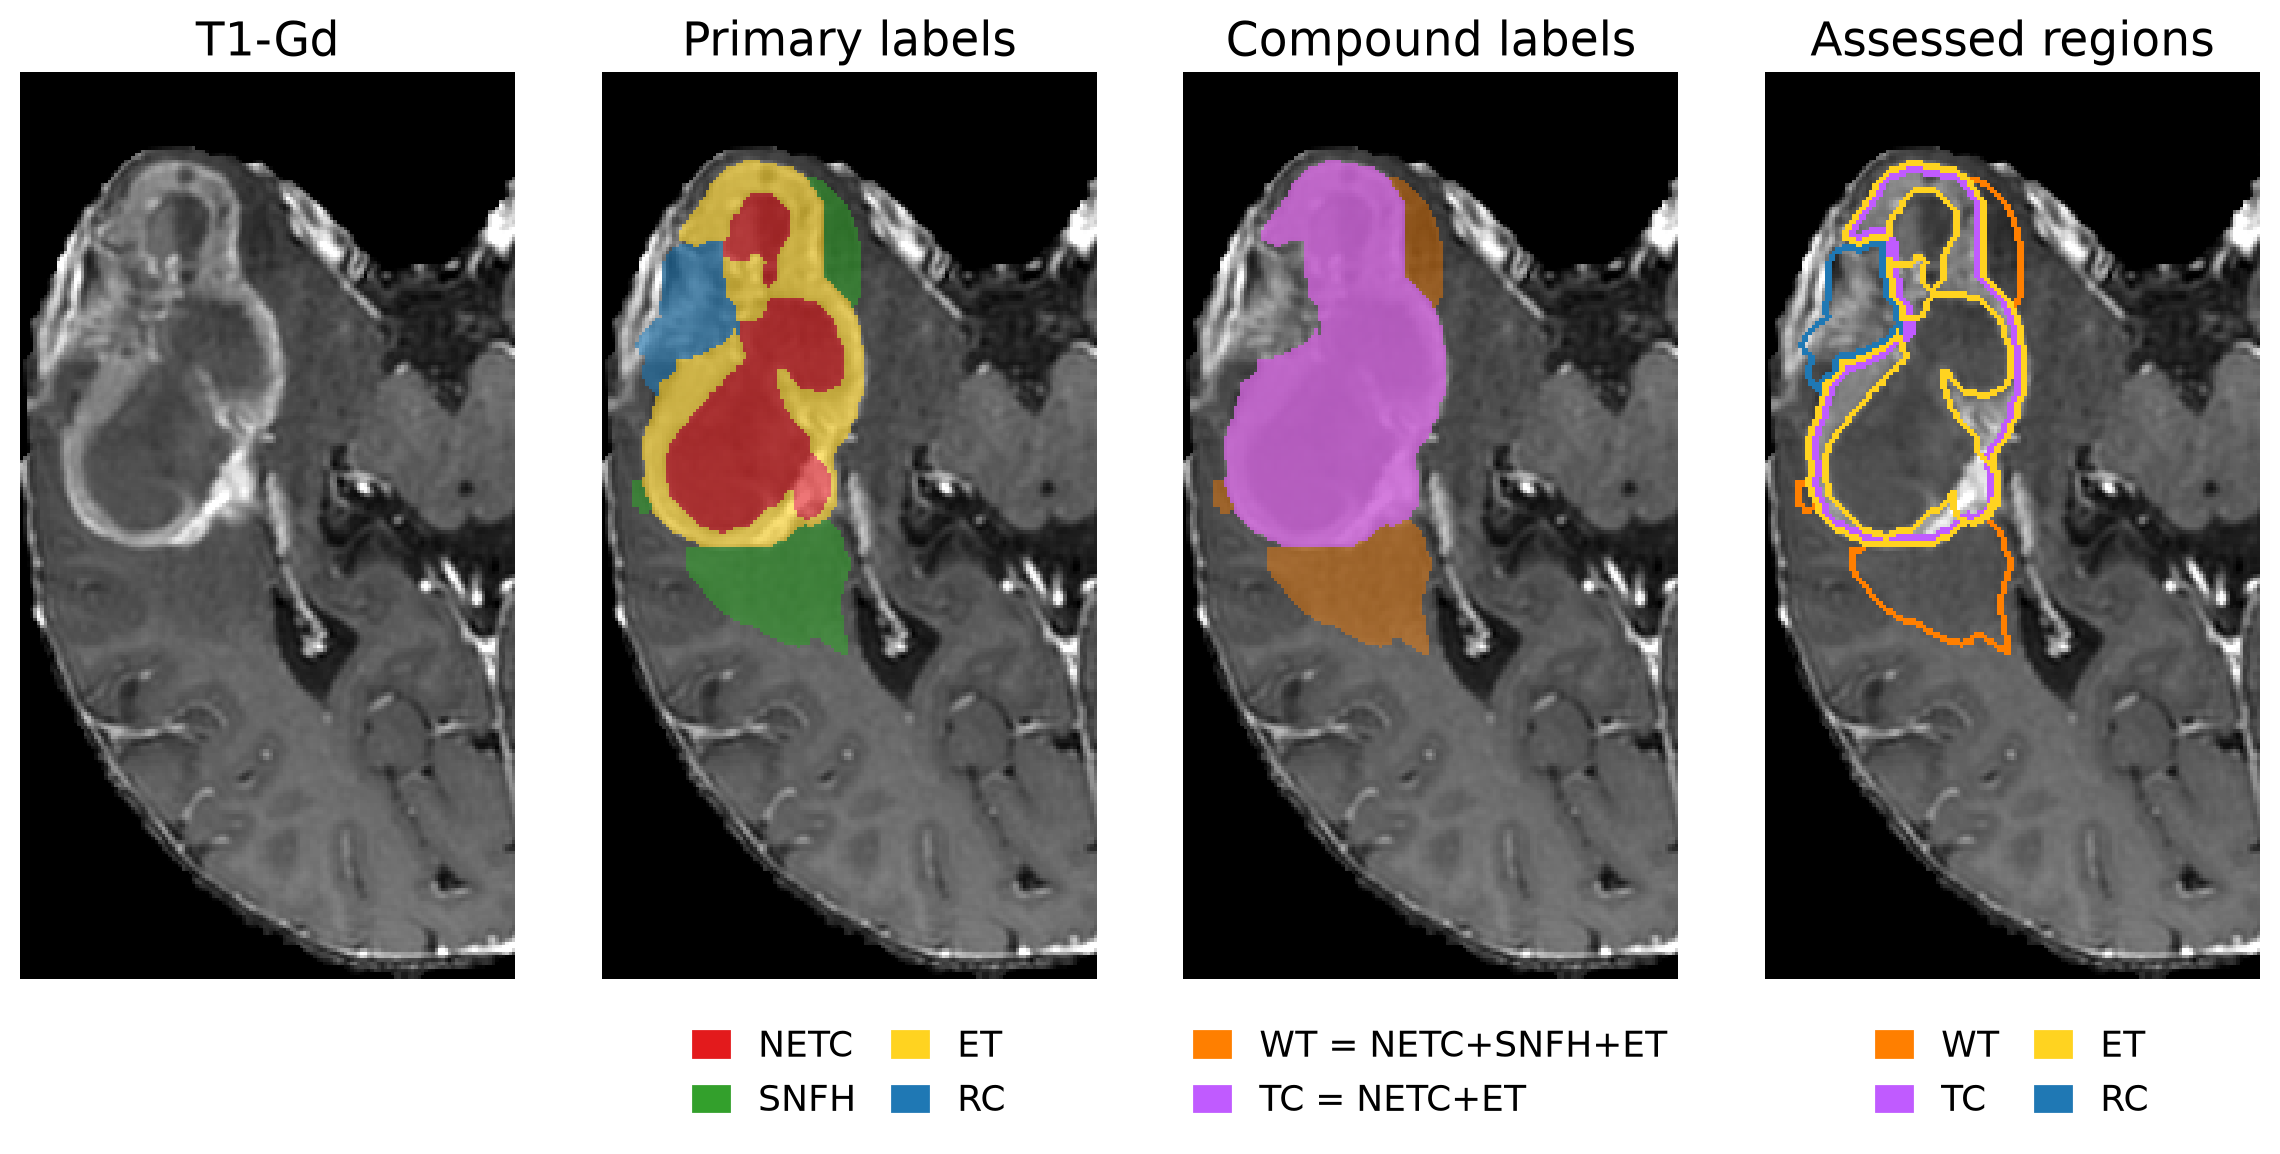
\includegraphics[height=0.72\textheight]{figures/labels_case.png}\\[0.4em]
\vspace{0.5em}
{\footnotesize\color{black!60}Training case sub-01321-002 \,$\cdot$\, scored as WT, TC, ET, RC \,$\cdot$\, RC present in only 13\% of cases}
\end{frame}

\begin{frame}{Metrics}
\centering
{\scriptsize\color{black!60}per case and region (\lab{WT}\; \lab{TC}\; \lab{ET}\; \lab{RC}) \,$\cdot$\, lesion = connected component \,$\cdot$\, matched 1:1 on any overlap}\\[0.8em]
\begin{tikzpicture}[
  box/.style={line width=1pt,rounded corners=4pt,text width=6.1cm,minimum height=4.3cm,align=left,anchor=north,inner sep=8pt},
]
  \node[box,draw=black!60,fill=black!4] at (0,0) {%
    \centering{\large\bfseries Lesion-wise DSC}\\[-0.1em]
    {\footnotesize\color{black!60}same scheme for NSD}\\[0.6em]
    \raggedright\footnotesize
    \textbullet\ Large GT lesions only ($\ge 20\,\mathrm{mm}^3$)\\[0.3em]
    \textbullet\ Matched $\rightarrow$ its DSC; missed $\rightarrow 0$\\[0.3em]
    \textbullet\ \textbf{Every FP component} adds a $0$\par\vspace{0.7em}
    \centering
    \makebox[\linewidth][c]{$\mathrm{DSC}_{\mathrm{lw}}=\dfrac{\sum_{\text{matched}}\mathrm{DSC}_i}{N_{\text{large}}+\mathrm{FP}}$}};
  \node[box,draw=kclred,fill=kclred!8] at (7.4,0) {%
    \centering{\large\bfseries Small-lesion $F_1$}\\[-0.1em]
    {\footnotesize\color{black!60}detection}\\[0.6em]
    \raggedright\footnotesize
    \textbullet\ Small GT lesions only ($<20\,\mathrm{mm}^3$)\\[0.3em]
    \textbullet\ TP if matched with DSC $\ge 0.1$, else FN\\[0.3em]
    \textbullet\ FP = \textbf{all} unmatched predictions, any size\par\vspace{0.7em}
    \centering
    \makebox[\linewidth][c]{$F_1=\dfrac{2\,\mathrm{TP}}{2\,\mathrm{TP}+\mathrm{FP}+\mathrm{FN}}$}};
\end{tikzpicture}\\[0.8em]
{\small A stray fragment is penalised \textbf{twice}: a $0$ in the DSC average and an FP in $F_1$}
\end{frame}

{\renewcommand{\slideref}{[1] S.\,S.~Kundu \emph{et al.}, ``Instance awareness of multi-class semantic segmentation loss functions,'' arXiv:2604.24276, 2026.}
\begin{frame}{Hillclimb Goal: Instance Awareness}
\centering
\vspace{1.2em}
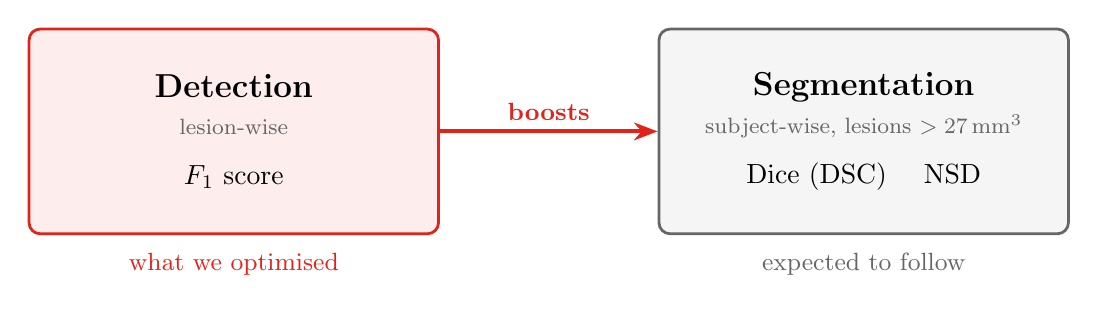
\begin{tikzpicture}[
  box/.style={line width=1pt,rounded corners=4pt,minimum width=5.2cm,minimum height=2.6cm,align=center},
]
  \node[box,draw=kclred,fill=kclred!8] (det) at (0,0) {%
    {\large\bfseries Detection}\\[0.15em]{\footnotesize\color{black!60}lesion-wise}\\[0.6em]
    $F_1$ score};
  \node[box,draw=black!60,fill=black!4] (seg) at (8,0) {%
    {\large\bfseries Segmentation}\\[0.15em]{\footnotesize\color{black!60}subject-wise, lesions $>27\,\mathrm{mm}^3$}\\[0.6em]
    Dice (DSC) \quad NSD};
  \draw[-{Stealth[length=3mm]},line width=1.5pt,kclred] (det.east) -- node[above,font=\small\bfseries]{boosts} (seg.west);
  \node[font=\small\color{kclred},anchor=north] at (det.south) [yshift=-0.3em] {what we optimised};
  \node[font=\small\color{black!60},anchor=north] at (seg.south) [yshift=-0.3em] {expected to follow};
\end{tikzpicture}
\vfill
We optimised for \textbf{instance awareness}~[1] through the detection task,\\
aiming to \textbf{automatically boost segmentation} performance.
\vspace{1.5em}
\end{frame}
}


{
\begin{frame}{Ensemble Candidates}
\centering
\vspace{-0.3em}
{\small\color{black!60}All three: nnU-Net ResEnc-L \texttt{3d\_fullres}, mirroring TTA}\\[0.2em]
{\small\color{black!60}Trained on all data: no local validation set created}\\[0.5em]
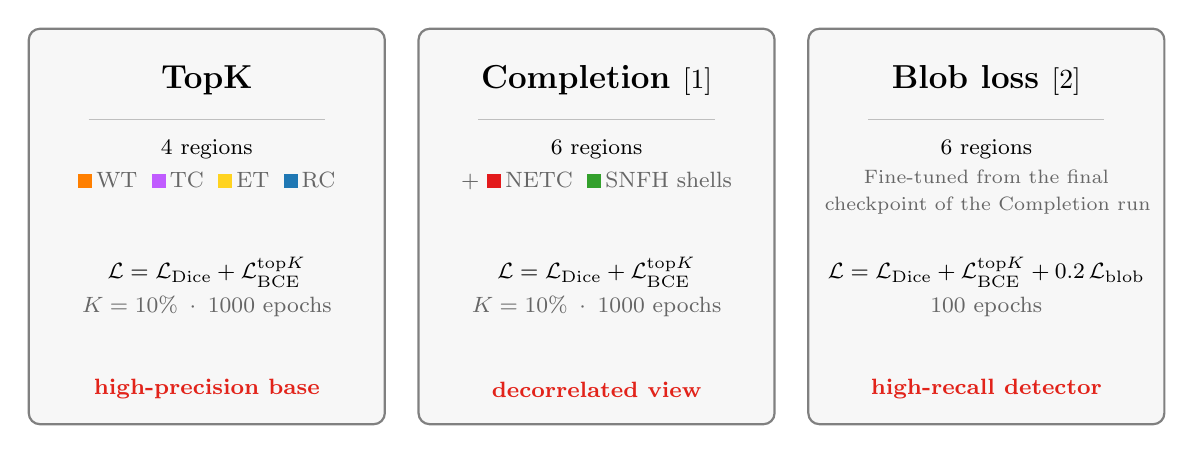
\begin{tikzpicture}[
  card/.style={draw=black!50,fill=black!3,line width=0.8pt,rounded corners=4pt,
    inner sep=6pt,anchor=north,font=\footnotesize},
]
  \node[card] at (0,0) {\begin{minipage}[t][4.6cm][t]{4.1cm}\centering
    \parbox[c][0.9cm][c]{4.1cm}{\centering\large\bfseries TopK}\\
    {\color{black!25}\rule{3cm}{0.4pt}}\\[0.35em]
    \parbox[t][1.45cm][t]{4.1cm}{\centering 4 regions\\[0.3em]{\color{black!60}\lab{WT}\; \lab{TC}\; \lab{ET}\; \lab{RC}}}\\
    \parbox[t][1.2cm][t]{4.1cm}{\centering $\mathcal{L}=\mathcal{L}_{\mathrm{Dice}}+\mathcal{L}_{\mathrm{BCE}}^{\mathrm{top}K}$\\[0.3em]{\color{black!60}$K=10\%$ \,$\cdot$\, 1000 epochs}}\\
    \parbox[b][0.9cm][c]{4.1cm}{\centering\bfseries\color{kclred}high-precision base}
  \end{minipage}};
  \node[card] at (4.95,0) {\begin{minipage}[t][4.6cm][t]{4.1cm}\centering
    \parbox[c][0.9cm][c]{4.1cm}{\centering\large\bfseries Completion~{\normalsize\mdseries[1]}}\\
    {\color{black!25}\rule{3cm}{0.4pt}}\\[0.35em]
    \parbox[t][1.45cm][t]{4.1cm}{\centering 6 regions\\[0.3em]{\color{black!60}+ \lab{NETC}\; \lab{SNFH} shells}}\\
    \parbox[t][1.2cm][t]{4.1cm}{\centering $\mathcal{L}=\mathcal{L}_{\mathrm{Dice}}+\mathcal{L}_{\mathrm{BCE}}^{\mathrm{top}K}$\\[0.3em]{\color{black!60}$K=10\%$ \,$\cdot$\, 1000 epochs}}\\
    \parbox[b][0.9cm][c]{4.1cm}{\centering\bfseries\color{kclred}decorrelated view}
  \end{minipage}};
  \node[card] at (9.9,0) {\begin{minipage}[t][4.6cm][t]{4.1cm}\centering
    \parbox[c][0.9cm][c]{4.1cm}{\centering\large\bfseries Blob loss~{\normalsize\mdseries[2]}}\\
    {\color{black!25}\rule{3cm}{0.4pt}}\\[0.35em]
    \parbox[t][1.45cm][t]{4.1cm}{\centering 6 regions\\[0.3em]{\scriptsize\color{black!60}\mbox{Fine-tuned from the final}\\\mbox{checkpoint of the Completion run}}}\\
    \parbox[t][1.2cm][t]{4.1cm}{\centering $\mathcal{L}=\mathcal{L}_{\mathrm{Dice}}+\mathcal{L}_{\mathrm{BCE}}^{\mathrm{top}K}+0.2\,\mathcal{L}_{\mathrm{blob}}$\\[0.3em]{\color{black!60}100 epochs}}\\
    \parbox[b][0.9cm][c]{4.1cm}{\centering\bfseries\color{kclred}high-recall detector}
  \end{minipage}};
\end{tikzpicture}
\begin{tikzpicture}[remember picture,overlay]
  \node[anchor=south west,inner sep=0pt,align=left,font=\tiny,text=black!60]
    at ([xshift=0.6em,yshift=0.5em]current page.south west) {[1] R.~Saluja \emph{et al.}, ``BackSplit: the importance of sub-dividing the background in biomedical lesion segmentation,'' CVPR, 2026.\\{}[2] F.~Kofler \emph{et al.}, ``blob loss: instance imbalance aware loss functions for semantic segmentation,'' IPMI, 2023.};
\end{tikzpicture}
\end{frame}
}

{\renewcommand{\slideref}{[1] S.\,S.~Kundu \emph{et al.}, ``Instance awareness of multi-class semantic segmentation loss functions,'' arXiv:2604.24276, 2026.}
\begin{frame}{Training}
\begin{columns}[t]
\begin{column}{0.5\textwidth}
{\small\bfseries Setup}\\[0.6em]
\begin{itemize}\setlength\itemsep{1.1em}\footnotesize
  \item Multi-label: one sigmoid per region, so an \lab{ET} voxel is also \lab{TC} and \lab{WT}
  \item 6-region: \lab{NETC} and \lab{SNFH} added as extra channels, dropped at inference
  \item Decoded in order \lab{WT} $\rightarrow$ \lab{TC} $\rightarrow$ \lab{ET} $\rightarrow$ \lab{RC}; inner regions overwrite outer
\end{itemize}
\end{column}
\begin{column}{0.46\textwidth}
{\small\bfseries Design decisions}\\[0.6em]
\begin{itemize}\setlength\itemsep{1.1em}\footnotesize
  \item Checkpointing based on pseudo-Dice
  \item Blob loss weight of 0.2 based on [1]
  \item $K=10\%$ is the nnU-Net TopK default
  \item 100 fine-tuning epochs based on a qualitative check of the loss curve
\end{itemize}
\end{column}
\end{columns}
\end{frame}
}

\begin{frame}{Resection Cavity: Handled Differently}
\begin{columns}[c]
\begin{column}{0.5\textwidth}
\centering
{\scriptsize\color{black!60}training set, 1295 cases \,$\cdot$\, components $>27\,\mathrm{mm}^3$}\\[0.6em]
\footnotesize
\renewcommand{\arraystretch}{1.3}
\setlength{\tabcolsep}{6pt}
\begin{tabular}{@{}lcc@{}}
\toprule
 & WT & RC \\
\midrule
cases with region & 1222 & 160 \\
single component & 31\% & \textbf{85\%} \\
2+ components & \textbf{69\%} & 15\% \\
5+ components & \textbf{31\%} & 1\% \\
median (max) comps & 3 (153) & 1 (5) \\
\bottomrule
\end{tabular}\\[1em]
{\footnotesize\textbf{Tumour:} many lesions {\color{kclred}$\rightarrow$ ensemble + hysteresis}}\\[0.3em]
{\footnotesize\textbf{RC:} one structure {\color{kclred}$\rightarrow$ single model, keep largest}}
\end{column}
\begin{column}{0.48\textwidth}
\begin{itemize}\setlength\itemsep{0.6em}\footnotesize
  \item Taken from the \textbf{Blob loss model alone}: no ensembling, no hysteresis
  \item Threshold at $0.5$, then keep the \textbf{largest component}
\end{itemize}
\vspace{1em}
\centering
{\scriptsize\color{black!60}official validation set, 179 cases}\\[0.5em]
\footnotesize
\renewcommand{\arraystretch}{1.3}
\begin{tabular}{@{}lccc@{}}
\toprule
RC & DSC & NSD & $F_1$ \\
\midrule
before & 0.581 & 0.474 & 0.000 \\
+ RC from Blob loss & \up{0.049} & \up{0.047} & \up{0.167} \\
\bottomrule
\end{tabular}\\[0.5em]
{\scriptsize\color{black!60}WT / TC / ET unchanged ($\le$0.001)}
\end{column}
\end{columns}
\end{frame}


\begin{frame}{Hysteresis Decoding}
\vspace{0.5em}
\begin{enumerate}\setlength\itemsep{1.2em}
  \item Threshold at $t_{\textsf{low}}=0.25$ and take the \textbf{connected components}
  \item For each component: is \textbf{any voxel above} $t_{\textsf{high}}=0.70$?
  \begin{itemize}\setlength\itemsep{0.5em}
    \item \textbf{No} $\rightarrow$ \textcolor{kclred}{\textbf{discard}} the whole component
    \item \textbf{Yes} $\rightarrow$ \textcolor{upgreen}{\textbf{keep}} the whole component (all its voxels above $0.25$)
  \end{itemize}
\end{enumerate}
\vspace{1em}
\begin{center}
\footnotesize
\renewcommand{\arraystretch}{1.3}
\begin{tabular}{@{}lll@{}}
\toprule
 & \textbf{Baseline:} single $t=0.5$ & \textbf{Hysteresis} \\
\midrule
Voxels kept & every voxel $>0.5$ & voxels $>0.25$, if peak $>0.70$ \\
Lesion margins ($0.25$--$0.5$) & \textcolor{kclred}{dropped (cut short)} & \textcolor{upgreen}{kept} \\
Weak blob (peak $0.52$) & \textcolor{kclred}{kept (false positive)} & \textcolor{upgreen}{discarded} \\
\bottomrule
\end{tabular}
\end{center}
\end{frame}

\begin{frame}{Hysteresis Decoding: Intuition}
\vspace{-0.8em}\begin{center}
\centering
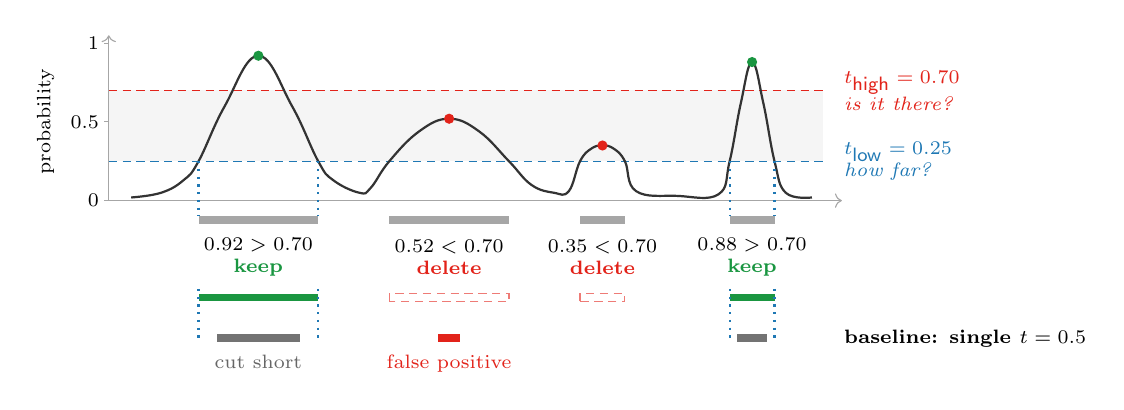
\begin{tikzpicture}[xscale=0.95, yscale=2.0]
\fill[black!4] (0,0.25) rectangle (9.55,0.70);
\draw[densely dashed,kclred] (0,0.70) -- (9.55,0.70);
\draw[densely dashed,cRC] (0,0.25) -- (9.55,0.25);
\node[font=\scriptsize,kclred,anchor=west,align=left] at (9.7,0.70) {$t_{\textsf{high}}=0.70$\\\emph{is it there?}};
\node[font=\scriptsize,cRC,anchor=west,align=left] at (9.7,0.25) {$t_{\textsf{low}}=0.25$\\\emph{how far?}};
\draw[->,gray!70] (0,0) -- (9.8,0);
\draw[->,gray!70] (0,0) -- (0,1.05);
\foreach \y/\l in {0/0, 0.5/0.5, 1.0/1}
  \draw[gray!70] (-0.06,\y) -- (0,\y) node[left,black,font=\scriptsize] {\l};
\node[rotate=90,font=\scriptsize,anchor=south] at (-0.6,0.5) {probability};
\draw[thick,black!80] plot[smooth,tension=0.7] coordinates {
  (0.30,0.02) (0.70,0.05) (1.00,0.13) (1.20,0.25) (1.55,0.60) (2.00,0.92)
  (2.45,0.60) (2.80,0.25) (3.00,0.13) (3.35,0.05)
  (3.50,0.08) (3.75,0.25) (4.15,0.44) (4.55,0.52) (4.95,0.44) (5.35,0.25)
  (5.65,0.10) (5.95,0.05)
  (6.15,0.06) (6.30,0.25) (6.45,0.33) (6.60,0.35) (6.75,0.33) (6.90,0.25)
  (7.05,0.06)
  (7.60,0.03) (8.15,0.04) (8.30,0.25) (8.45,0.62) (8.60,0.88) (8.75,0.62)
  (8.90,0.25) (9.05,0.05) (9.40,0.02) };
\foreach \x/\y/\c in {2.00/0.92/upgreen, 4.55/0.52/kclred, 6.60/0.35/kclred, 8.60/0.88/upgreen}
  \node[circle,fill=\c,inner sep=1.3pt] at (\x,\y) {};
\fill[black!35] (1.20,-0.15) rectangle (2.80,-0.10);
\fill[black!35] (3.75,-0.15) rectangle (5.35,-0.10);
\fill[black!35] (6.30,-0.15) rectangle (6.90,-0.10);
\fill[black!35] (8.30,-0.15) rectangle (8.90,-0.10);
\fill[upgreen] (1.20,-0.64) rectangle (2.80,-0.59);
\draw[kclred!60,densely dashed] (3.75,-0.64) rectangle (5.35,-0.59);
\draw[kclred!60,densely dashed] (6.30,-0.64) rectangle (6.90,-0.59);
\fill[upgreen] (8.30,-0.64) rectangle (8.90,-0.59);
\node[font=\scriptsize,align=center] at (2.00,-0.36) {$0.92>0.70$\\\textcolor{upgreen}{\bfseries keep}};
\node[font=\scriptsize,align=center] at (4.55,-0.36) {$0.52<0.70$\\\textcolor{kclred}{\bfseries delete}};
\node[font=\scriptsize,align=center] at (6.60,-0.36) {$0.35<0.70$\\\textcolor{kclred}{\bfseries delete}};
\node[font=\scriptsize,align=center] at (8.60,-0.36) {$0.88>0.70$\\\textcolor{upgreen}{\bfseries keep}};
% extent guides: where each kept blob crosses t_lo
\foreach \x in {1.20,2.80,8.30,8.90}
  {\draw[cRC,dotted,thick] (\x,0.25) -- (\x,-0.10); \draw[cRC,dotted,thick] (\x,-0.56) -- (\x,-0.90);}
% contrast: one global threshold at 0.5
\fill[black!55] (1.45,-0.90) rectangle (2.55,-0.85);
\fill[kclred] (4.40,-0.90) rectangle (4.70,-0.85);
\fill[black!55] (8.40,-0.90) rectangle (8.80,-0.85);
\node[font=\scriptsize\bfseries,anchor=west] at (9.7,-0.875) {baseline: single $t=0.5$};
\node[font=\scriptsize,kclred,anchor=north] at (4.55,-0.92) {false positive};
\node[font=\scriptsize,black!60,anchor=north,align=center] at (2.00,-0.92) {cut short};
\end{tikzpicture}\\[0.2em]

\end{center}
\end{frame}

\begin{frame}{Primary Ablation}
\centering
{\scriptsize\color{black!60}official validation set, 179 cases \,$\cdot$\, each row: change vs.\ the row above}\\[0.5em]
\scriptsize
\renewcommand{\arraystretch}{1.25}
\setlength{\tabcolsep}{3.2pt}
\begin{tabular}{@{}l cccc c cccc@{}}
\toprule
 & \multicolumn{4}{c}{DSC} & & \multicolumn{4}{c}{$F_1$} \\
\cmidrule(lr){2-5}\cmidrule(lr){7-10}
configuration & WT & TC & ET & RC & & WT & TC & ET & RC \\
\midrule
Single model & 0.560 & 0.622 & 0.593 & -- &  & 0.379 & 0.469 & 0.463 & --  \\
+ 2-model ensemble & \up{0.106} & \up{0.086} & \up{0.091} & 0.556$^\dagger$ &  & \dn{0.011} & \dn{0.030} & \dn{0.027} & 0.000$^\dagger$  \\
+ 2-model ensemble (Completion) & \up{0.012} & \up{0.010} & \up{0.012} & \up{0.025} &  & \up{0.002} & \up{0.038} & \up{0.048} & {\color{black!50}0.000}  \\
+ RC from Blob loss & \up{0.001} & \up{0.001} & {\color{black!50}0.000} & \up{0.049} &  & {\color{black!50}0.000} & {\color{black!50}0.000} & {\color{black!50}0.000} & \up{0.167}  \\
+ Hysteresis (0.40 / 0.60) & \up{0.032} & \up{0.034} & \up{0.033} & {\color{black!50}0.000} &  & \dn{0.005} & \dn{0.009} & \dn{0.009} & {\color{black!50}0.000}  \\
{\color{black!60}\quad\emph{alt.}\ 0.30 / 0.70$^\ddagger$} & \up{0.041} & \up{0.042} & \up{0.041} & {\color{black!50}0.000} &  & \up{0.006} & \up{0.002} & \dn{0.007} & {\color{black!50}0.000}  \\
{\color{black!60}\quad\emph{alt.}\ 0.25 / 0.70$^\ddagger$} & \up{0.046} & \up{0.047} & \up{0.050} & {\color{black!50}0.000} &  & \up{0.006} & \up{0.001} & \dn{0.008} & {\color{black!50}0.000}  \\
+ 3-model ensemble & \up{0.009} & \up{0.008} & \up{0.008} & {\color{black!50}0.000} &  & \up{0.011} & \up{0.011} & \up{0.002} & {\color{black!50}0.000}  \\
+ Hysteresis (0.25 / 0.70) & \up{0.005} & \up{0.005} & \up{0.009} & {\color{black!50}0.000} &  & {\color{black!50}0.000} & \dn{0.001} & \dn{0.001} & {\color{black!50}0.000}  \\
\midrule
\textbf{final} & \textbf{0.725} & \textbf{0.766} & \textbf{0.746} & \textbf{0.630} &  & \textbf{0.376} & \textbf{0.478} & \textbf{0.476} & \textbf{0.167} \\
\bottomrule
\end{tabular}\\[0.4em]
{\tiny\color{black!60}$^\dagger$first RC score available (single-model RC not recorded) \,$\cdot$\, $^\ddagger$alternative thresholds, change vs.\ the row before hysteresis}
\end{frame}

\begin{frame}{Takeaways}
\vspace{1em}
\begin{itemize}\setlength\itemsep{1.4em}
  \item Most \underline{prior work} acquires instance awareness \underline{during training}. Our objective was to be instance aware during inference as well.
  \item Knowing \underline{which labels} need instance awareness is also key: applied to a label that is usually one structure (RC), instance-aware techniques hurt rather than help.
  \item \textbf{\underline{There is a clear need to adopt instance-aware evaluation schemes.}}
\end{itemize}
\end{frame}

\begin{frame}[plain]
\vfill
\begin{center}
{\Huge\bfseries Thank you}\\[0.6em]
{\color{kclred}\rule{0.2\textwidth}{1.5pt}}
\end{center}
\vfill
\end{frame}

\end{document}
